\subsubsection{Heurística constructiva de cluster-first, route-second, clusterizando con algoritmo de K-means}

\subsubsubsection{Medición en base a tamaño del grafo}

Al no depender de n, si no de la distribución de los puntos y sus respectivas demandas, se espera un gráfico con variaciones.

\begin{figure}[H]
	\centering
	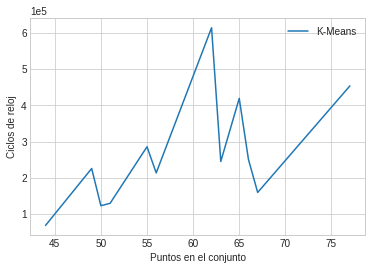
\includegraphics[scale=0.6]{exercise5/kmeans3.png}
\end{figure}

Tal como era de esperar, el gráfico no presenta una curva de crecimiento continuo a medida que crece el valor de n. Es fácil visualizar los distintos altos y bajos en el gráfico y por ende resulta trivial concluir que la distribución de los puntos es aquello que afecta a la heurística K-means.